\chapter*{Ход работы}

\section*{Код по общему заданию}
Код программы по общему заданию представлен на листинге 1.

\FloatBarrier
\begin{lstinputlisting}[caption=Код общего задания, 
	linerange={1, 33}, basicstyle=\footnotesize\ttfamily, frame=single, breaklines=true]{src/common.s}
\end{lstinputlisting}
\FloatBarrier

Дизассемблированный код представлен на листинге 2

\FloatBarrier
\begin{lstinputlisting}[caption=Дизассемблированный код общего задания, 
	linerange={1, 41}, basicstyle=\footnotesize\ttfamily, frame=single, breaklines=true]{src/common.obj}
\end{lstinputlisting}
\FloatBarrier

Псевдокод на языке С представлен на листинге 3.
\FloatBarrier
\begin{lstinputlisting}[caption=Псевдокод общего задания, 
	linerange={1, 24}, basicstyle=\footnotesize\ttfamily, frame=single, breaklines=true]{src/common.c}
\end{lstinputlisting}
\FloatBarrier

\section*{Задание 2}

Задание: получить снимок экрана, содержащий временную диаграмму выполнения стадий выборки и диспетчеризации команды с указанным адресом.

Мой вариант: 6. 

Адрес команды, номер итерации: 80000020, 1-я.

Код команды: 002f8fb3.

Команда: add x31,x31,x2.


Во время выборки команды снимается сигнал gc\_fetch\_hold разрешая работу блока выборки, а сигнал pc\_id\_available равен 1,
что подтверждает готовность блока управления метаданными принять результат выборки. 
Сигнал pc равен адресу команды, также этот адрес выставляется на шину данных (addr).

Выставление сигнала en разрешает работу памяти команд. Одновременно с этим выставляется сигнал pc\_id\_assigned, указывающий блоку управления метаинформацией,
что запрос в память отправлен, и информация о текущем pc должна быть записана в очередь команд.
В начале следующего такта значение pc будет записано в pc\_table по индексу, равному значению текущего первого свободного id, а
pc\_id увеличится на 1.


По фронту, завершающему такт 2, выбраный код команды (то есть, сигнал fetch\_instruction) записывается
в таблицу instruction\_table по индексу. Это завершает операцию диспетчеризации.

На рисунке 1 приведён скрин по заданию с подписанными соответствующими сигналами:
\FloatBarrier
\begin{figure}[h]
	\begin{center}
		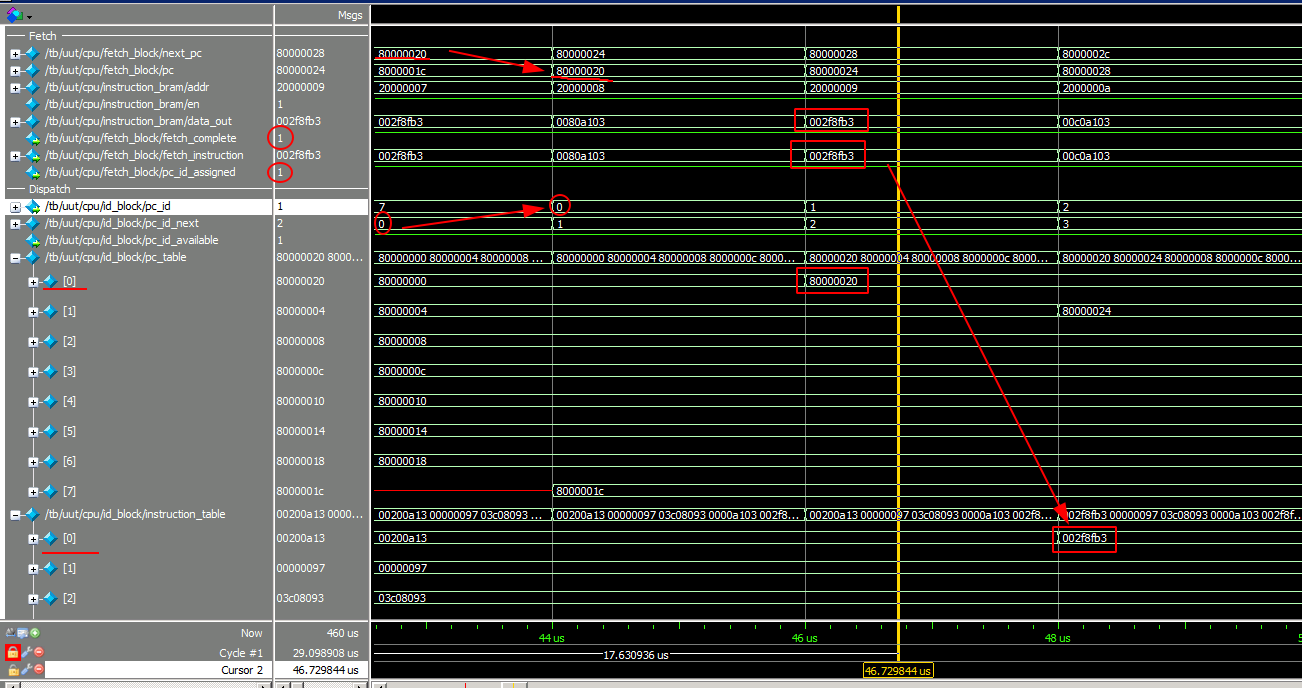
\includegraphics[width=\linewidth, height=10cm]{inc/first_ex.png}
	\end{center}
	\caption{Демонстрация выборки и диспетчеризации команды}
\end{figure}
\FloatBarrier


\section*{Задание 3}
Задание: получить снимок экрана, содержащий временную диаграмму выполнения стадии декодирования и планирования на выполнение команды с указанным адресом. 

Мой вариант: 6.

Адрес команды, номер итерации: 8000002с, 1-я. 

Код команды: 01008093.

Команда: addi x1,x1,16.

Так как возник конфликт по регистру x1 (rs2), выполнение стадии декодирования заняло 3 такта, а не один.
Из-за конфликта сигнал decode\_advance выставлен в 0.

На рисунке 2 приведён скрин по заданию с подписанными соответствующими сигналами:
\FloatBarrier
\begin{figure}[h]
	\begin{center}
		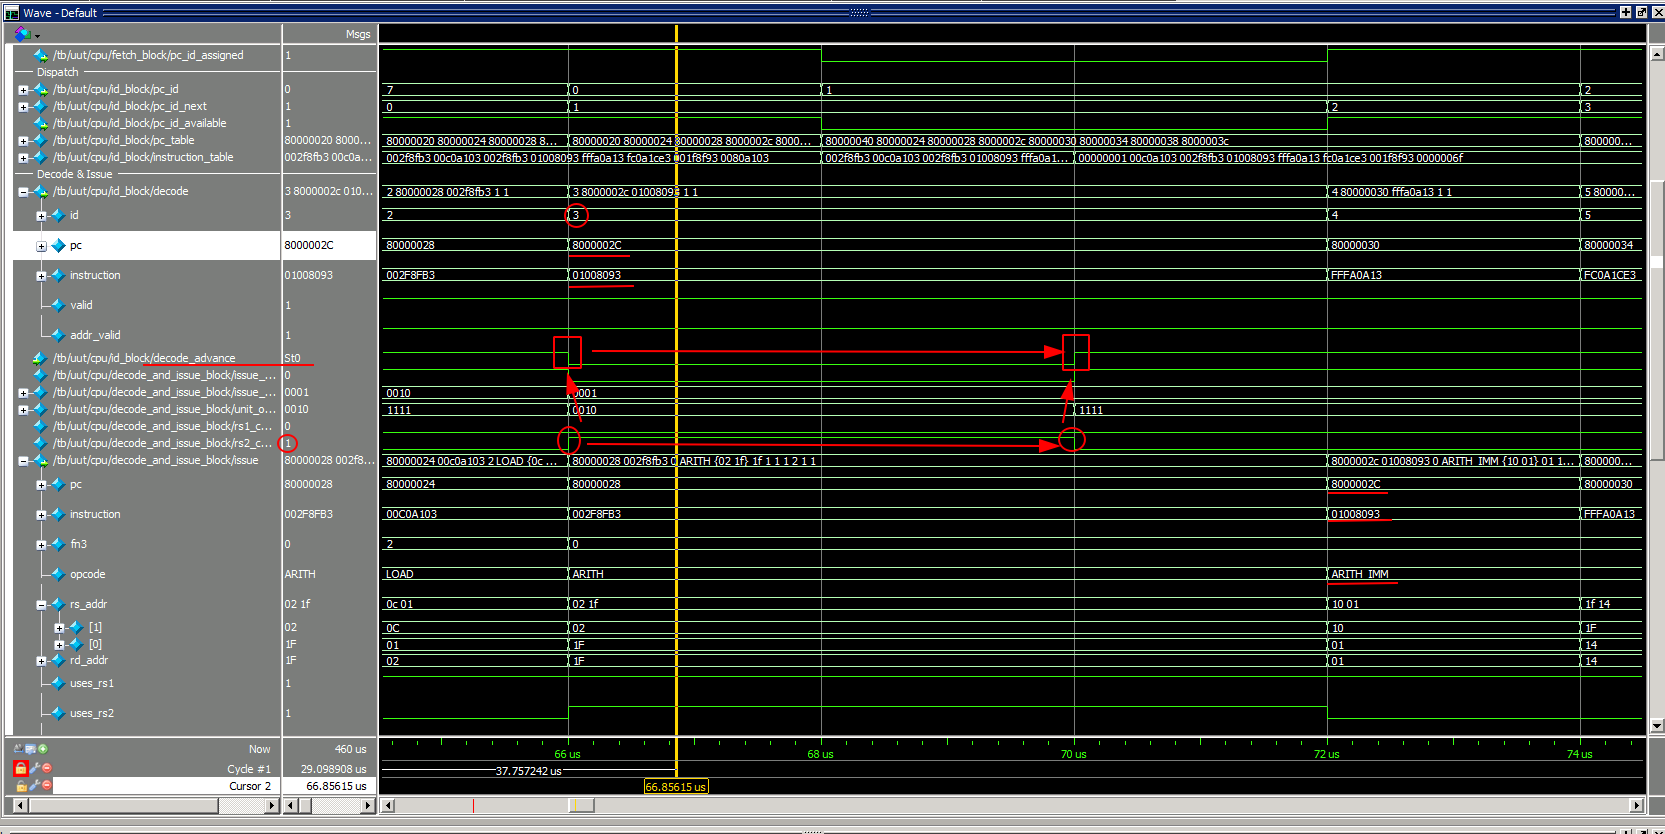
\includegraphics[width=\linewidth, height=10cm]{inc/second_ex.png}
	\end{center}
	\caption{Демонстрация выполнения стадии декодирования и планирования}
\end{figure}
\FloatBarrier

\section*{Задание 4}

Задание: получить снимок экрана, содержащий временную диаграмму выполнения стадии выполнения команды с указанным адресом.
Мой вариант: 6.

Адрес команды, номер итерации: 80000014, 1-я.

Код команды: 0040a103. 

Команда: lw x2,4(x1).

Это команда блока обращения к памяти, поэтому выполнение заняло 3 такта.

На рисунках 3-4 приведены скрины по заданию с подписанными соответствующими сигналами:
\FloatBarrier
\begin{figure}[h]
	\begin{center}
		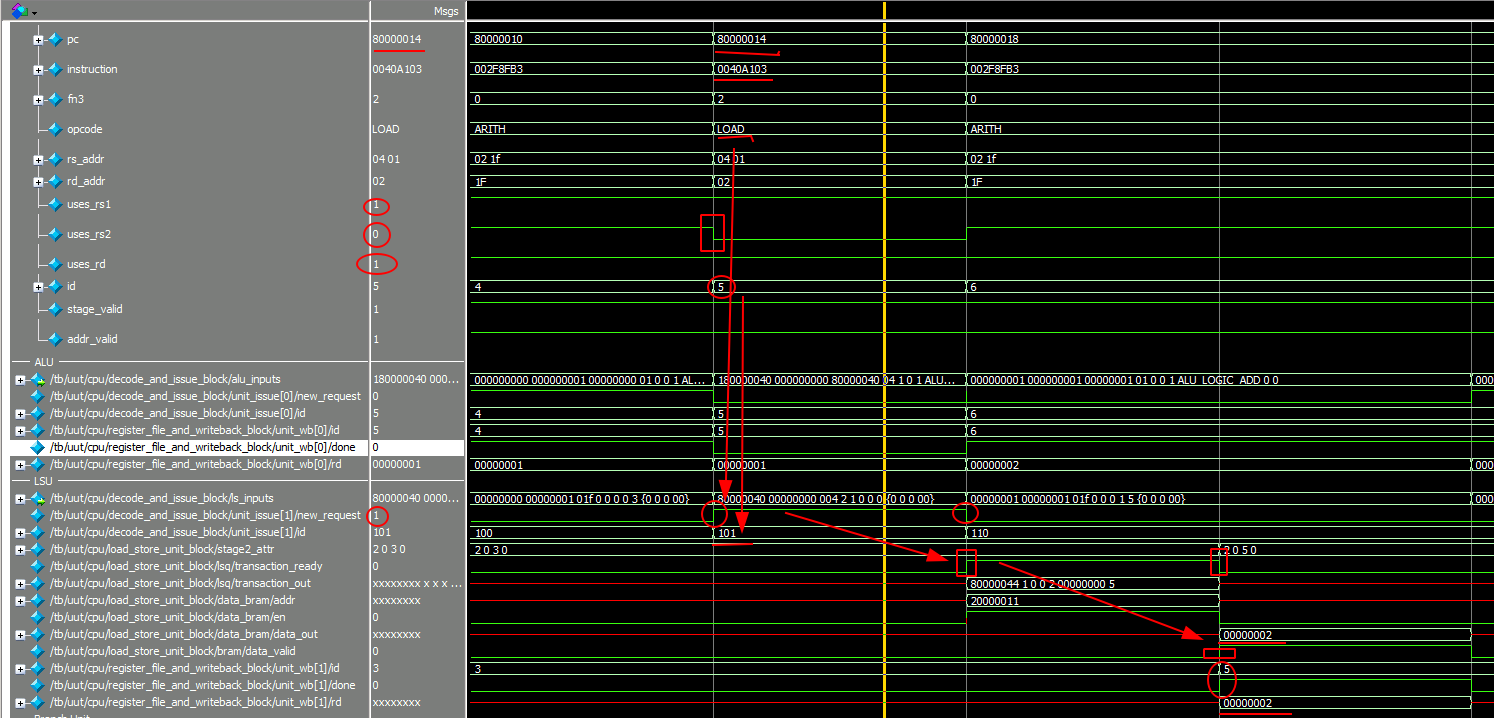
\includegraphics[width=\linewidth, height=12cm]{inc/third_ex_1.png}
	\end{center}
	\caption{Демонстрация выполнения стадии выполнения программы (часть 1)}
\end{figure}
\FloatBarrier

\FloatBarrier
\begin{figure}[h]
	\begin{center}
		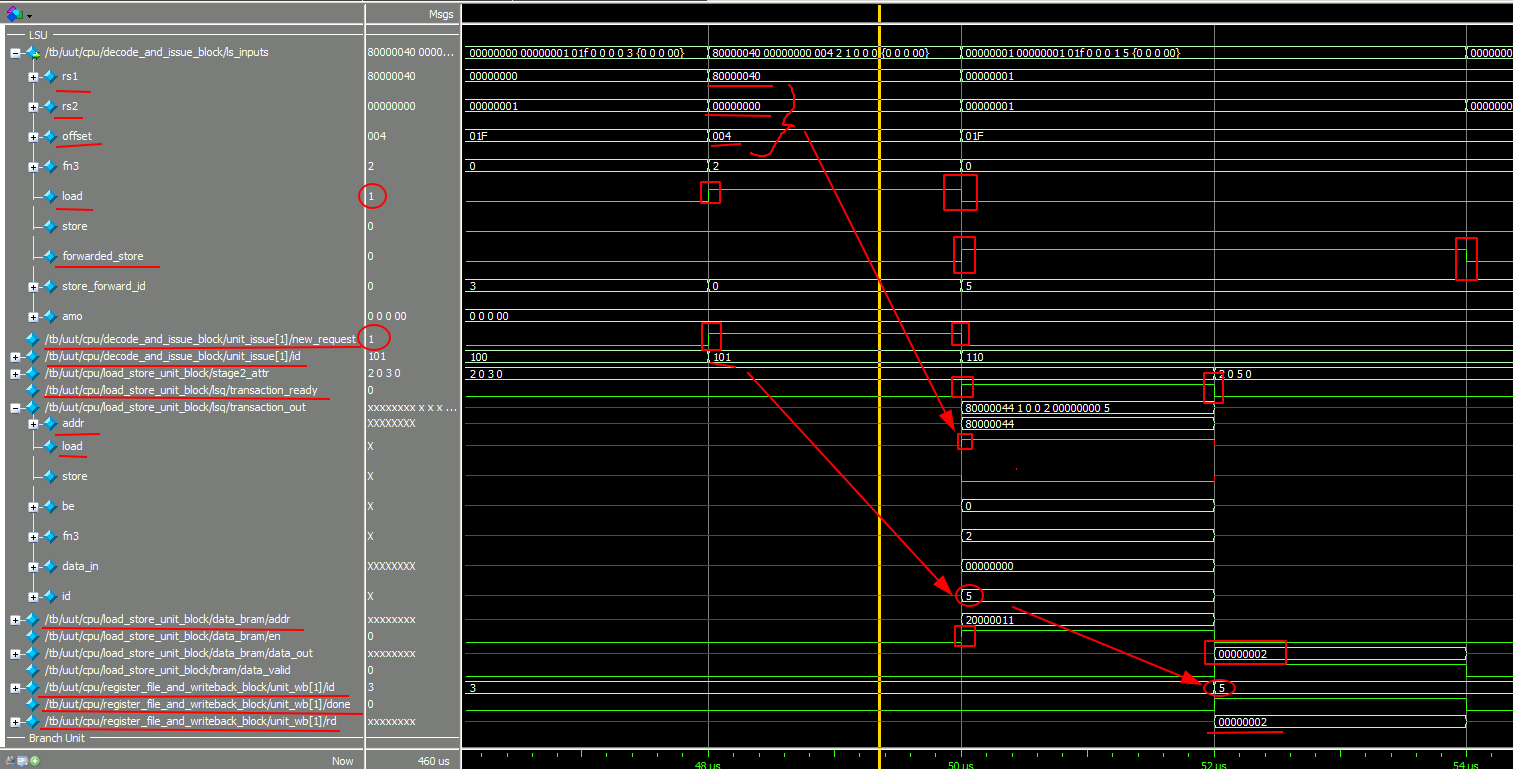
\includegraphics[width=\linewidth, height=12cm]{inc/third_ex_2.png}
	\end{center}
	\caption{Демонстрация выполнения стадии выполнения программы (часть 2)}
\end{figure}
\FloatBarrier

\section*{Код по индивидуальному заданию}
Код программы по индивидуальному заданию представлен на листинге 4.

\FloatBarrier
\begin{lstinputlisting}[caption=Код индивидуального задания, 
	linerange={1, 33}, basicstyle=\footnotesize\ttfamily, frame=single, breaklines=true]{src/my_prog.s}
\end{lstinputlisting}
\FloatBarrier

Дизассемблированный код представлен на листинге 5:

\FloatBarrier
\begin{lstinputlisting}[caption=Дизассемблированный код индивидуального задания, 
	linerange={1, 41}, basicstyle=\footnotesize\ttfamily, frame=single, breaklines=true]{src/my_prog.obj}
\end{lstinputlisting}
\FloatBarrier


\section*{Задание 5}
Была получена временную диаграмму сигналов выполнения программы индивидуального варианта.

На рисунке 5 показан результат работы программы, который содержится в регистре x31:
\FloatBarrier
\begin{figure}[h]
	\begin{center}
		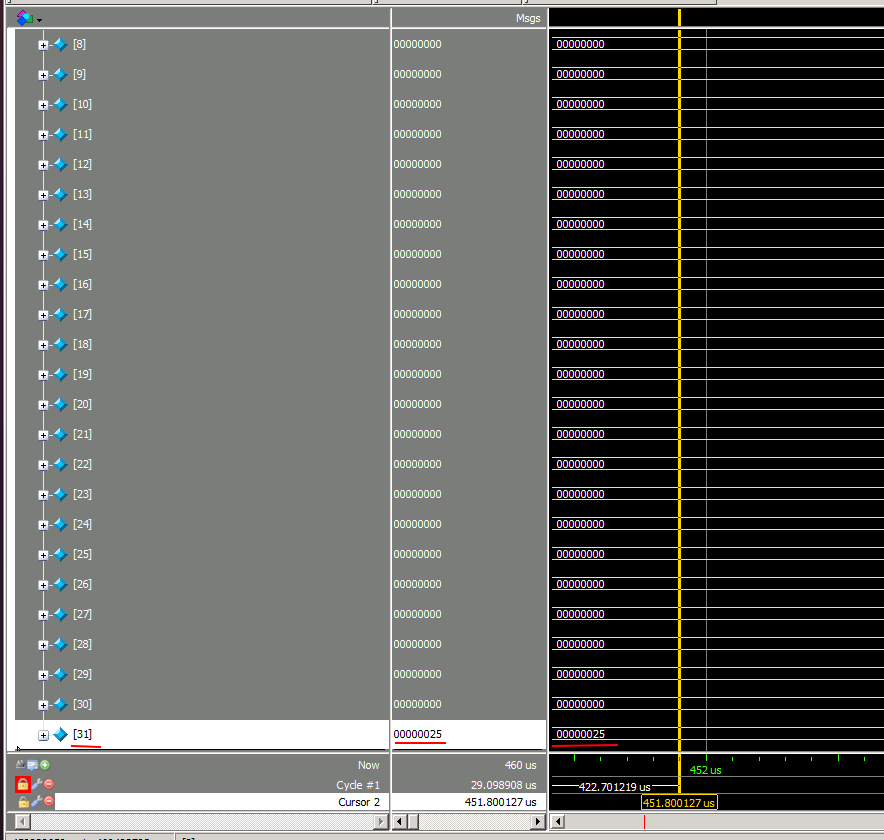
\includegraphics[width=\linewidth, height=10cm]{inc/result_my.png}
	\end{center}
	\caption{Результат работы программы}
\end{figure}
\FloatBarrier

Результат совпал с ожидаемым.

Задание: Получить снимок экрана, содержащий временные диаграммы сигналов, соответствующих всем стадиям выполнения команды, обозначенной в тексте программы символом !.

Мой вариант -- 6.

Адрес команды: 80000010. 

Код команды: 0040a183. 

Команда: lw x3, 4(x1).

На рисунке 6 показан скрин выполнения стадий выборки и диспетчеризации для команды:
\FloatBarrier
\begin{figure}[h]
	\begin{center}
		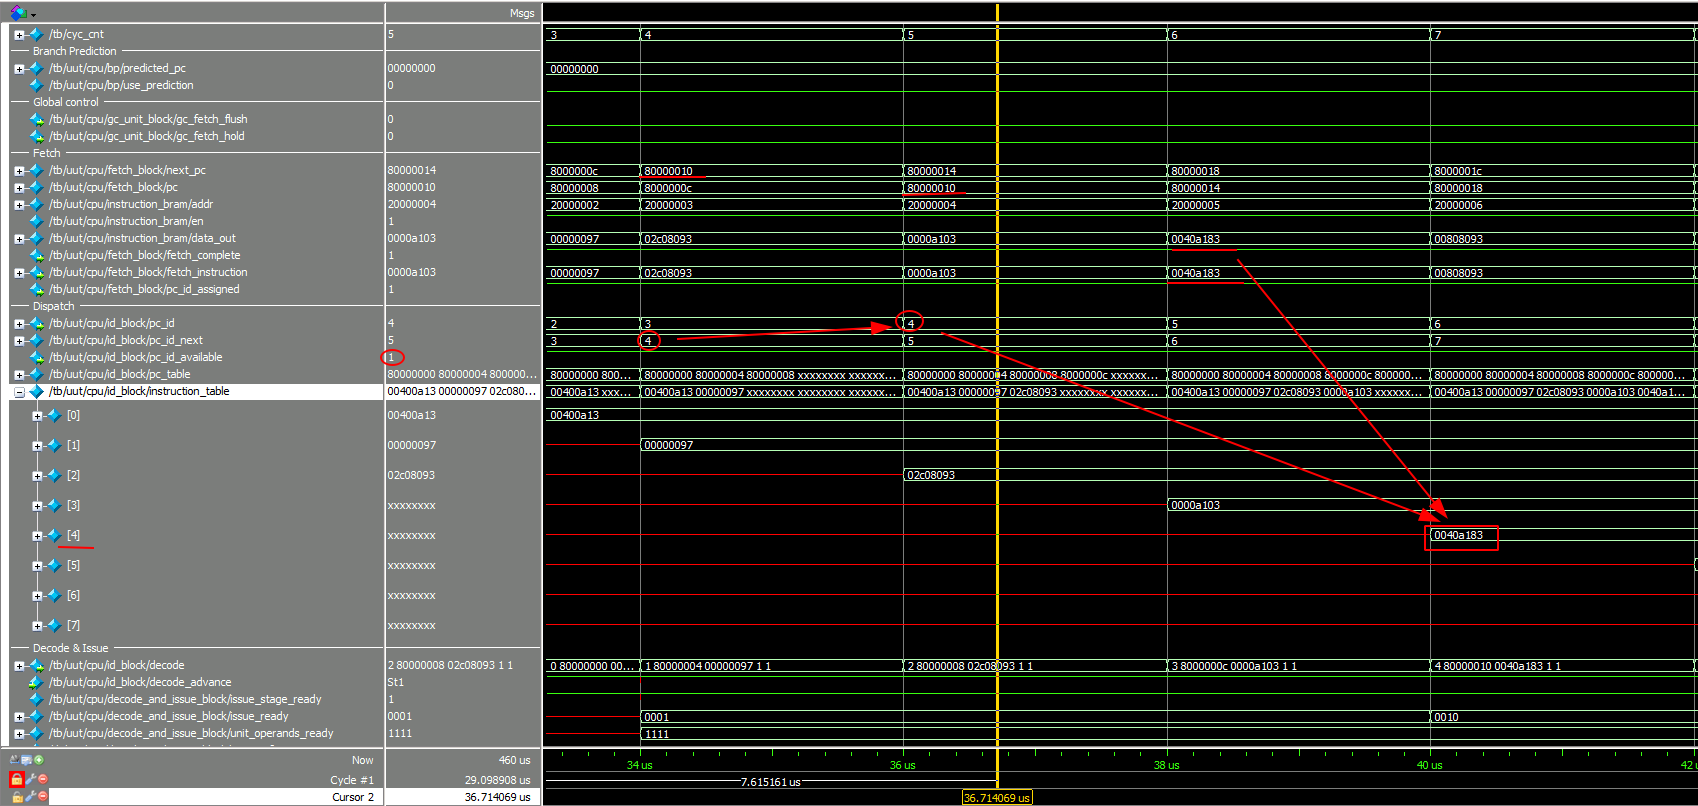
\includegraphics[width=\linewidth, height=7.5cm]{inc/first_my.png}
	\end{center}
	\caption{Демонстрация выполнения стадий выборки и диспетчеризации для команды по индивидуальному варианту}
\end{figure}
\FloatBarrier

На рисунке 7 показан скрин выполнения стадий декодирования и планирования для команды:
\FloatBarrier
\begin{figure}[h]
	\begin{center}
		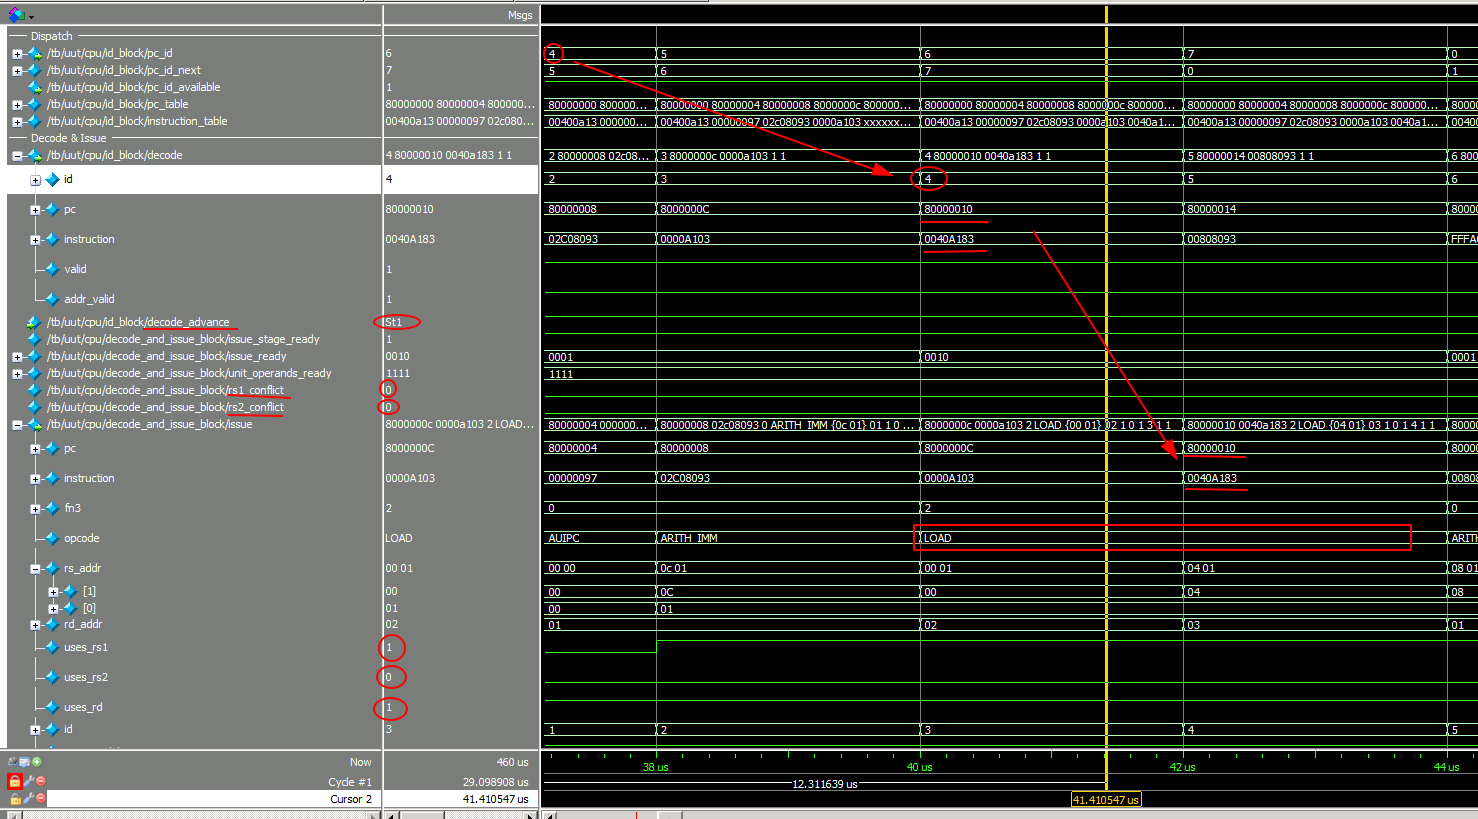
\includegraphics[width=\linewidth, height=7.5cm]{inc/second_my.png}
	\end{center}
	\caption{Демонстрация выполнения стадий декодирования и планирования для команды по индивидуальному варианту}
\end{figure}
\FloatBarrier

На рисунках 8-9 показаны скрины выполнения стадии выполнения для команды:
\FloatBarrier
\begin{figure}[h]
	\begin{center}
		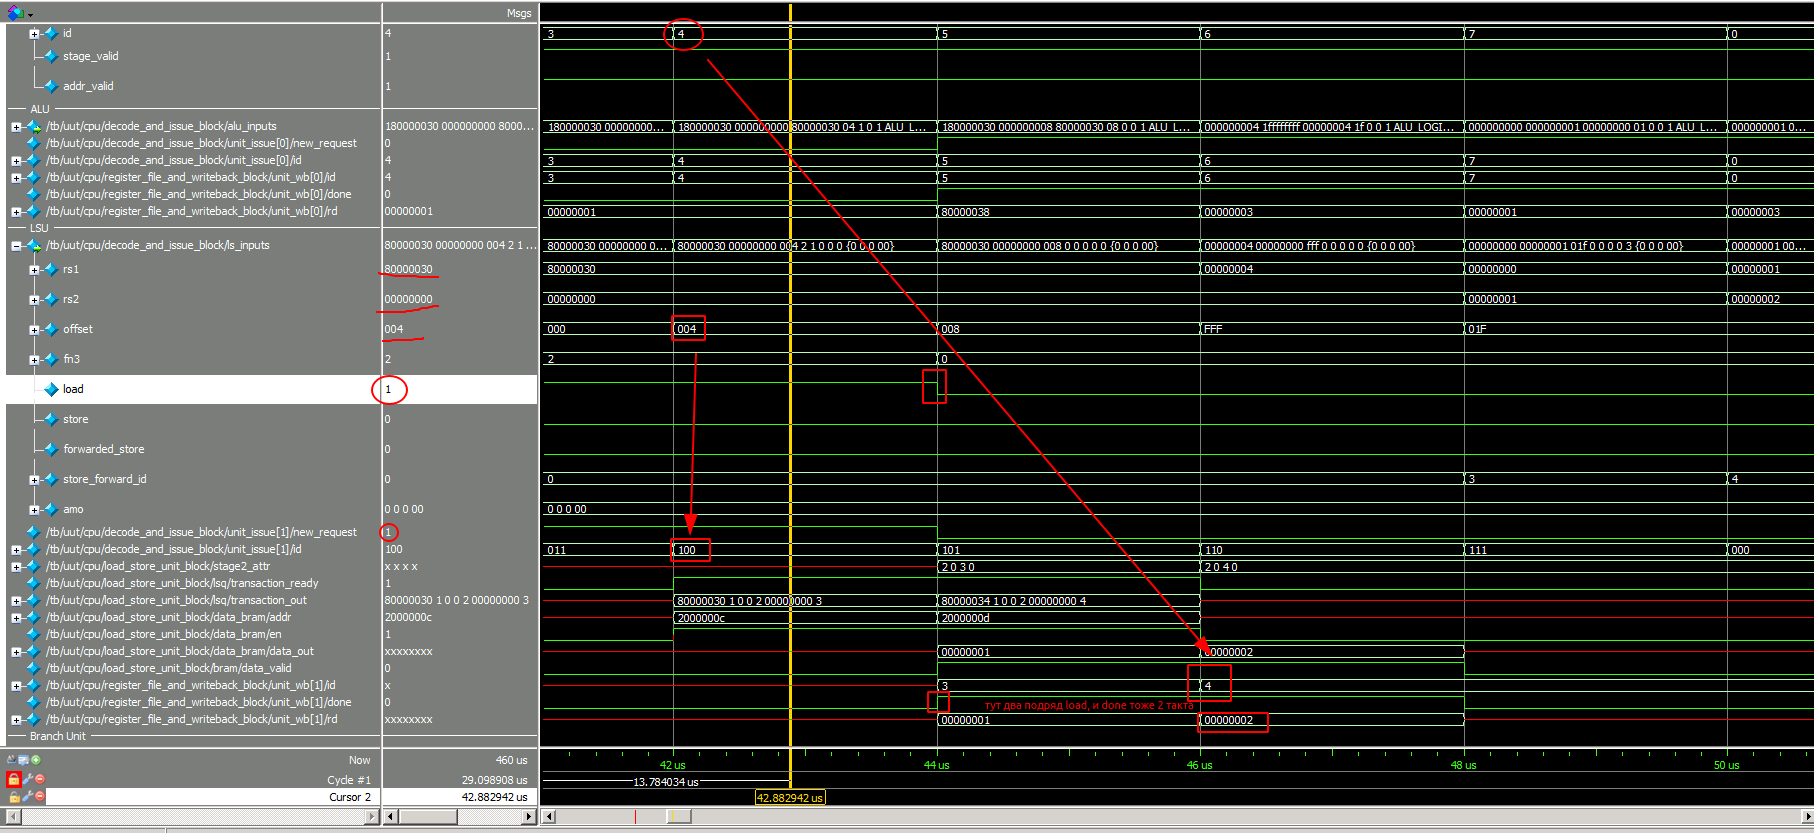
\includegraphics[width=\linewidth, height=10cm]{inc/third_my.png}
	\end{center}
	\caption{Демонстрация выполнения стадии выполнения для команды по индивидуальному варианту (часть 1)}
\end{figure}
\FloatBarrier

\FloatBarrier
\begin{figure}[h]
	\begin{center}
		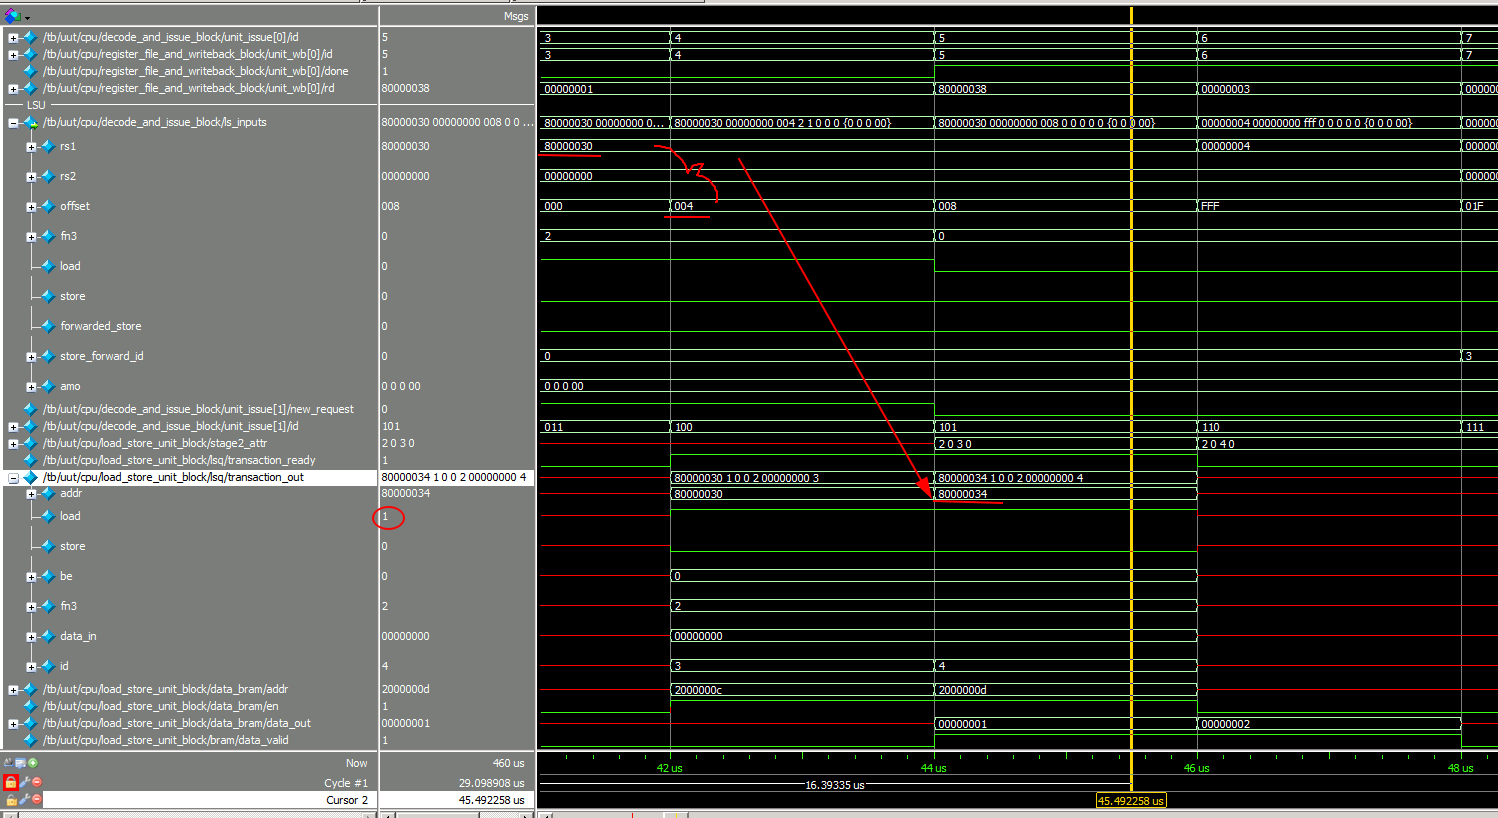
\includegraphics[width=\linewidth, height=10cm]{inc/third_1_my.png}
	\end{center}
	\caption{Демонстрация выполнения стадии выполнения для команды по индивидуальному варианту (часть 2)}
\end{figure}
\FloatBarrier

\section*{Трасса выполнения программы}
На рисунке 10 приведена трасса выполнения программы:
\FloatBarrier
\begin{figure}[h]
	\begin{center}
		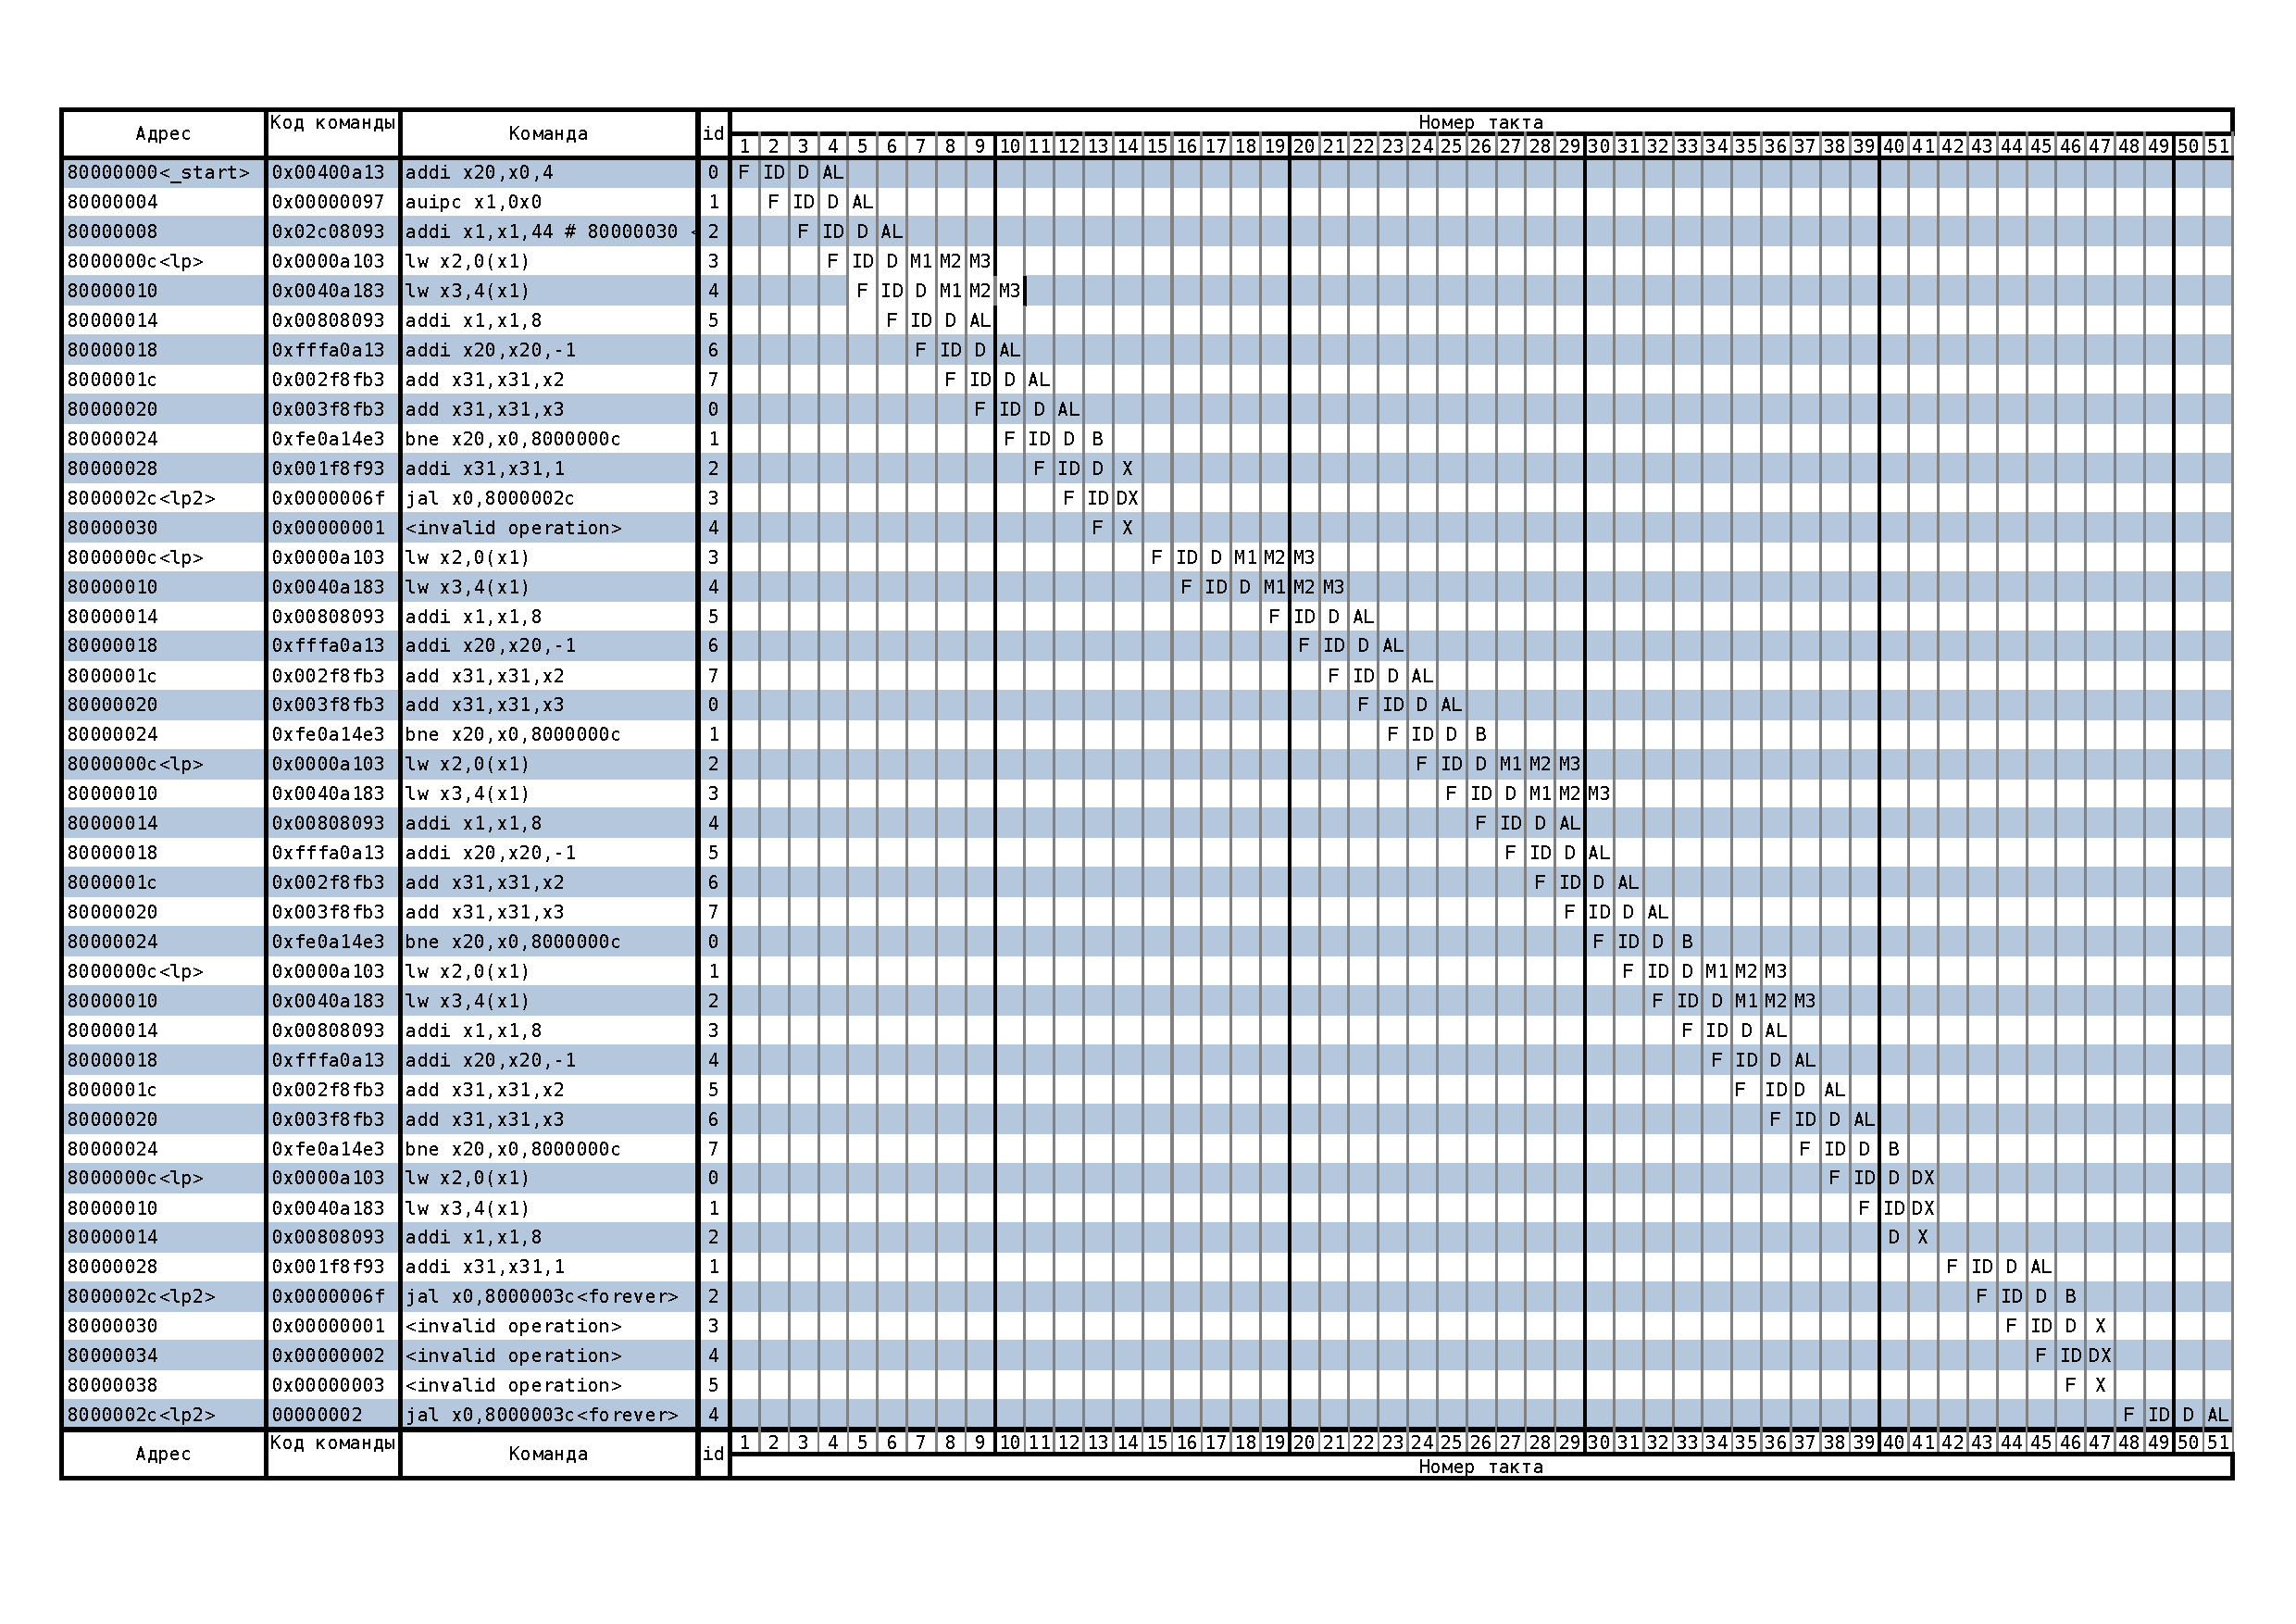
\includegraphics[width=\linewidth, height=16cm]{inc/my_ex.pdf}
	\end{center}
	\caption{Трасса выполнения программы}
\end{figure}
\FloatBarrier

Конфликтов по операндам в программе не было, но программа дважды неправильно угадывала результат сравнения в цикле, из-за чего выполнение было дольше.

\section*{Оптимизация программы}
Так как задержка шла из-за циклов, я принял решение убрать цикл.
Программа считает сумму всех элементов массива, поэтому я сначала все значения массива в регистр, а затем сложил их и получил ответ.

Код программы по общему заданию представлен на листинге 6.

\FloatBarrier
\begin{lstinputlisting}[caption=Оптимизированный код индивидуального задания, 
	linerange={1, 33}, basicstyle=\footnotesize\ttfamily, frame=single, breaklines=true]{src/opt.s}
\end{lstinputlisting}
\FloatBarrier

Дизассемблированный код представлен на листинге 7:

\FloatBarrier
\begin{lstinputlisting}[caption=Дизассемблированный код, 
	linerange={1, 41}, basicstyle=\footnotesize\ttfamily, frame=single, breaklines=true]{src/opt.obj}
\end{lstinputlisting}
\FloatBarrier

На рисунке 11 представлен результат работы программы:
\FloatBarrier
\begin{figure}[h]
	\begin{center}
		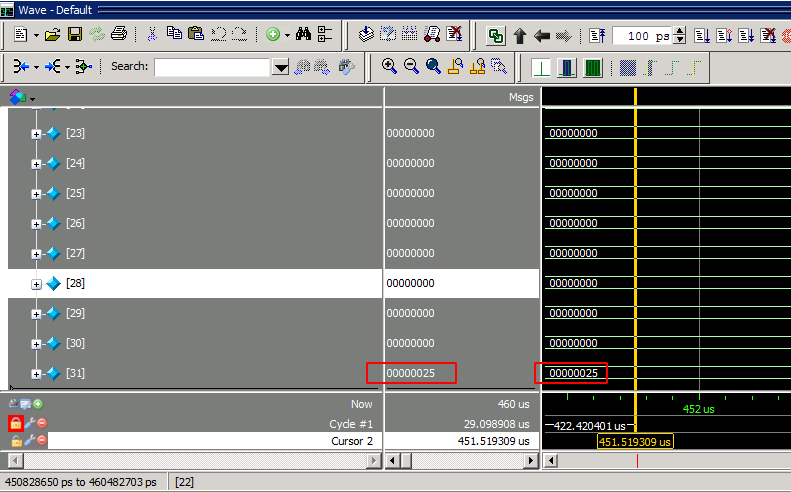
\includegraphics[width=\linewidth, height=10cm]{inc/opt_result.png}
	\end{center}
	\caption{Результат работы оптимизированной программы}
\end{figure}
\FloatBarrier

Результат совпал с ожидаемым и полученным для начальной программы.

На рисунке 12 представлена трасса выполнения оптимизированной программы
\FloatBarrier
\begin{figure}[h]
	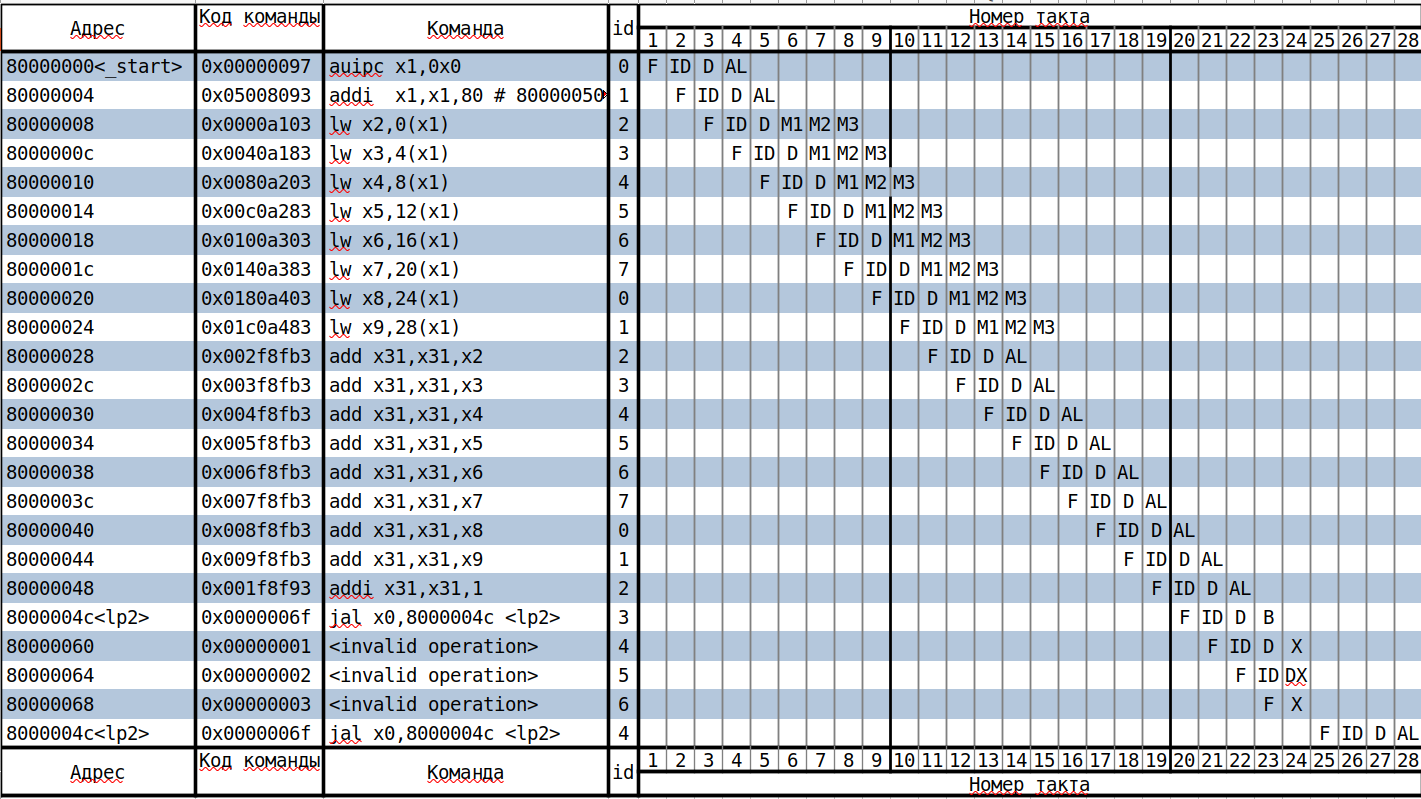
\includegraphics[width=\linewidth]{inc/opt.png}
	\caption{Трасса выполнения оптимизированной программы}
\end{figure}
\FloatBarrier

Количество тактов сокращено практически вдвое. Цена — расширяемость
программы.

\section*{Вывод}
В результате выполнения лабораторной работы были изучены принципы
функционирования, построения и особенности архитектуры суперскалярных
конвейерных микропроцессоров. Также были рассмотрены принципы
проектирования и верификации сложных цифровых устройств с использованием
языка описания аппаратуры SystemVerilog и ПЛИС. На основе изученных
материалов был найден способ оптимизации программы. 